\subsection{A. Personnel Qualifications List}
\begin{itemize}
\item Chief Technology Officer (CTO): 		Kai Braungardt
\item Chief Executive Officer (CEO): 		Moritz Gimpel-Henning
\item Chief Financial Officer (CFO): 		Annabelle Engelhardt
\item Chief Administrative Officer (CAO): 	Christian Geier
\item Chief Operating Officer (COO): 		Lennart Knipper
\end{itemize}

\includepdf[pages=-, pagecommand={}]{Lebenslauf_Kai}

\includepdf[pages=-, pagecommand={}]{Lebenslauf_Moritz}
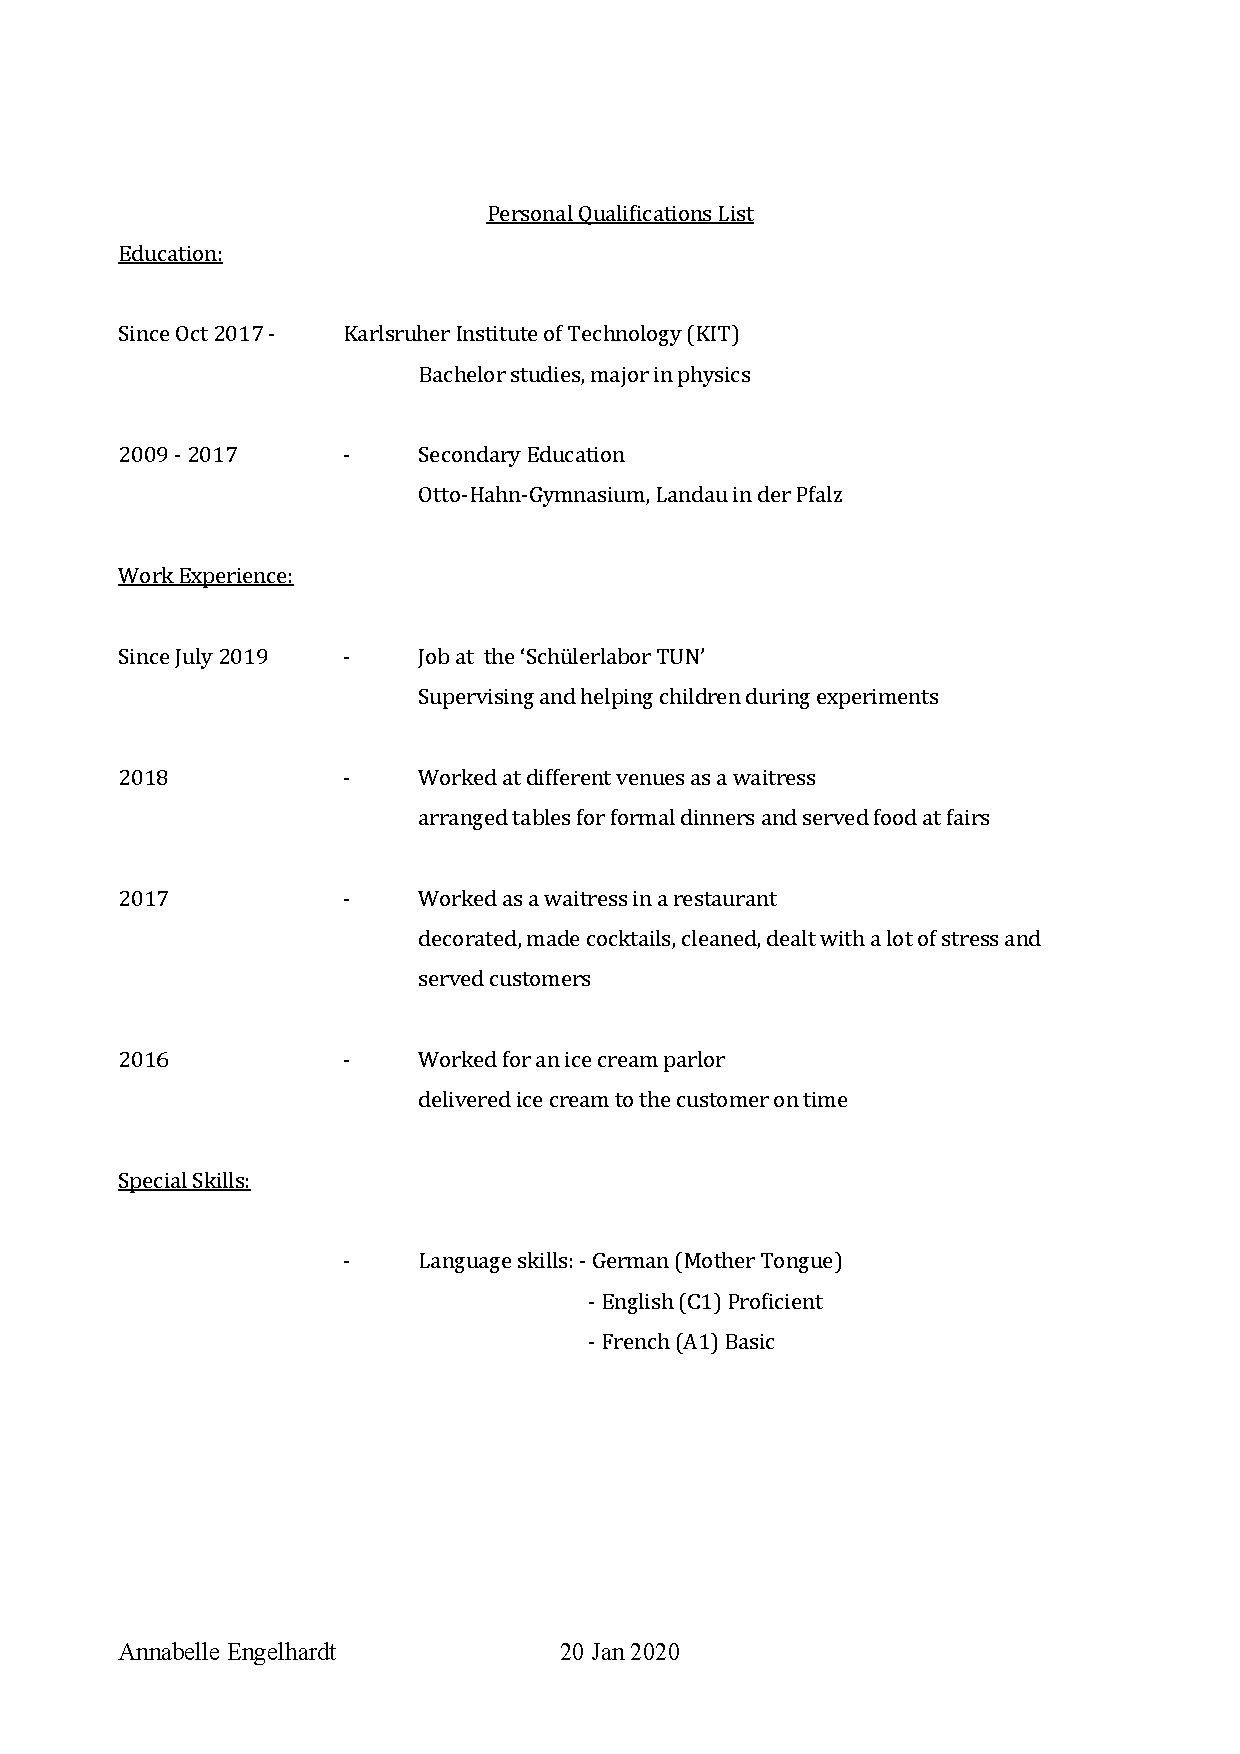
\includepdf[pages=-, pagecommand={}]{SectionVI_A_Annabelle}

\includepdf[pages=-, pagecommand={}]{Lebenslauf_Christian}

\includepdf[pages=-, pagecommand={}]{Lebenslauf_Lennart}

\subsection{B. Resources}
\begin{parcolumns}[colwidths={1=5 cm, 2=10 cm}]{2}

\colchunk{\\
\textbf{Vehicle to Grid}
\\ \\ \\ \\ \\ \\ \\ \\ \\ \\ 
\textbf{Pumped Storage Hydropower}
\\ \\ \\ \\ \\ \\ \\ \\ \\ \\
\textbf{Hydrogen as an Energy Storage System}
\\ \\ \\ \\ \\ \\ \\
\textbf{Power to Gas}
\\ \\ \\ \\ \\ \\ \\ \\
\textbf{Batteries}
}

\colchunk{\\
\url{https://en.wikipedia.org} \\ \url{https://www.isi.fraunhofer.de} \\ \url{https://www.erneuerbar-mobil.de} \\ \url{https://www.bdew.de} \\ \url{https://www.kba.de} \\ \url{https://de.statista.com} \\ \url{https://www.volkswagenag.com} \\ \url{https://backend.orbit.dtu.dk} \\ \url{https://www.bmwi.de/}
\\
\\ \url{https://en.wikipedia.org} \\ \url{https://www.bdew.de} \\ \url{https://www.hydropower.org} \\ \url{https://www.energy.gov} \\ \url{https://www.tep.com} \\ \url{https://www.lazard.com} \\ \url{https://books.google.co.uk} \\ \url{https://phys.org} \\ \url{https://www.ifc.org}
\\
\\ \url{https://www.researchgate.net} \\ \url{https://en.wikipedia.org} \\ \url{https://www.irena.org} \\ \url{https://www.azocleantech.com} \\ \url{https://www.hydrogenics.com} \\ \url{https://www.nrel.gov} \\ \url{https://publications.jrc.ec.europa.eu}
\\
\\ \url{https://en.wikipedia.org} \\ \url{https://www.bdew.de} \\ \url{https://www.elsevier.com} \\ \url{https://www.dena.de} \\ \url{https://www.sciencedirect.com} \\ \url{https://www.oxfordenergy.org} \\ \url{http://epub.sub.uni-hamburg.de}
\\
\\ \url{https://energystorage.org} \\ \url{https://circuitdigest.com} \\ \url{https://www.wikipedia.org} \\ \url{https://www.nature.com} \\ \url{http://www.energiefirmen.de} \\ \url{https://batteryuniversity.com} \\ \url{https://solarbay.com.au} \\
}

\end{parcolumns}
\clearpage

%%%%%%%%%%%%%%%%%%%%%%%%
\subsection{C. Costing}
\begin{parcolumns}[colwidths={1=2.5 cm, 2=10 cm, 3=2.5 cm}]{3}

\colchunk{\\ \textbf{Manhours}}

\colchunk{\\ 
The manhours are split into two categories. Work done individually, such as research and technical writing, is mentioned in total work hours. Work done together, such as team meetings, the work done on the presentation and hours spent in class, is mentioned in hours per person. At a rate of 12.50 € per person per hour the total costs for manhours comes to 3,650 €.
}

\colchunk{\\}

\end{parcolumns}

\begin{table}[H]
\centering
\caption{Total Manhours}
\begin{tabular}{cc}
\toprule
Manhours-Type & Hours \\
\midrule
Time in Class & 24h p.p. \\
Research & 37h \\
Technical Writing & 45h \\
Team meetings & 15h p.p. \\
Presentation & 3h p.p. \\
\bottomrule
\end{tabular}
\end{table}


\begin{parcolumns}[colwidths={1=2.5 cm, 2=10 cm, 3=2.5 cm}]{3}
\colchunk{\\ \textbf{Total Costs} }

\colchunk{\\ 
Printing costs are split into two parts. The costs per page of a one-sided black and white print at the AStA printing office is 0.03 €. The cost of the plastic binding is 0.50 €. This results in a total of 2.87 € for the entire paper. \\ \\
\noindent
The cost of 1 kWh in Germany is 0.30 €. At an average of 0.5 kW used per computer the cost of computing per hour is set to 0.15 €. This adds up to 25.8 € with the mentioned total manhours. \\ \\
\noindent
In total this results in 3,678.67 € for this paper.
}

\colchunk{\\}
\end{parcolumns}


\begin{table}[H]
\centering
\caption{Total Costs of Research Paper}
\begin{tabular}{cc}
\toprule
Cost-Type & Cost \\
\midrule
Manhours & 3,650.00 €\\
Computing Costs & 25.80 €\\
Printing Costs & 2.87 €\\
\bottomrule
\end{tabular}
\end{table}